\section{Four new distributions} \label{s4} 

\ssn{Learning Outcomes}
After studying this week you will be able to:
\begin{itemize}
\item use the geometric distribution to calculate probabilities;
\item explain what is meant by a continuous random variable and how it is represented by a probability density function;
\item compute probabilities and expectations for continuous random variables;
\item model appropriate problems using exponential or uniform distributions.
\end{itemize}
\end{n}

\subsection{Preparation for the week}

\ssn{Motivating problem} 
I have a process which, independently I execute it, has a probability $p$ of success. Let $X$ be the number of tries up to and including my first success. What is the probability that $\PP(X=k)$, i.e.\ I succeed for the first time on my $k$-th try. 

Setting $q=1-p$, to succeed on the $k$-th attempt, I have to fail $k-1$ times in a row and then succeed. Since the tries are all independent, we have 
 \[
         \PP(X=k) = q^{k-1} p. 
  \] 
\end{n}

\ssn{Definition: Geometric random variable} 
A random variable $X$ is \ul{geometric} and we write $X \sim \mathop{Geom}(p)$ if \hfill 
 \tcb 
   \[
         \PP(X=k) = q^{k-1} p \quad \text{where $q=1-p$.} 
  \] 
 \etcb
\end{n} 

\ssn{Proposition}  The expected value of $X \sim  \mathop{Geom}(p)$ is $\EE(X) = 1/p$. 
\begin{proof}
From the definition of $\EE(X)$ we have 
 \[
     \EE(X) = p + 2pq + 3pq^2 + 4 pq^3 + \dots .
 \]
Multiplying by $q$ we have 
 \[
      q \EE(X) = pq + 2pq^2 + 3pq^3 +  \dots .
 \]
 Subtracting
  \[
  (1-q) \EE(X) = p \EE(X) =  p + pq + pq^2 + pq^3 + \dots = \frac{p}{1-q} = 1.
  \]
 where we have summed the GP and used $q=1-p$. 
\end{proof}
\end{n}

\ssn{Example} 
 Suppose I roll a pair of D6 repeatedly I and count the number of rolls until I roll a total of `5'.  The probability of rolling a total of five is $4/36 = 1/9$. 
 
 So with $X \sim \mathop{Geom}(1/9)$ we have that the probability of succeeding first on the third roll is 
  \[
       \PP(X = 3) = q^2 p = \left( \frac89 \right)^2   \frac19 = 
       \frac{64}{729}.
  \]
  The expected number of rolls is $\EE(X) = 1/p = 9$. 
\end{n} 

\sse{Exercise} 
One day each week I go fishing in a lake and  I independently have a probability of $1/52$ of catching the big carp that lives there.
Let $X=k$ if I first catch the carp on my $k$-th day fishing. 
\begin{enumerate}
    \item On which day of fishing am I most likely to catch the carp? 
    \item What is the probability that I first catch the carp on my third day fishing? 
    \item What is the expected number of fishing days until I catch the carp? 
\end{enumerate}
\end{e}

\sss
Here $X \sim \mathop{Geom}(1/52)$. The value of $\PP(X=k)$ is greatest when $k=1$ and so the first day is the most probable day that I catch the fish.  The probability of first catching it on day 3 is $(51/52)^2 (1/52)$.  The expected number of days is $1/p$ = $52$. 
\end{s} 


\ssn{Exponential distribution: Motivating problem}
Radioactive atoms spontaneously decay after a certain time by emitting a particle.  It works like this. If the atom has not yet decayed at a given moment, then the probability of its decaying in the next short time $\Delta t$ is (in the limit as $\Delta t \map 0$) equal to $\lambda \Delta t$ where $\lambda$ is a constant for the particular type of atom. It does not matter if the atom in question has been around for millennia or if it was created a second ago, the chances of its decaying in the next second are the same.  So if we say we have an intact atom now at time $t=0$ what can we say about the probability of its decaying within a certain time?  
\end{n}

\ssn{The problem} 
We have a random variable $T$ here with sample space $[0,\infty)$, with the point $t$ corresponding to decay at time exactly $t$.  What is the probability of decay at time exactly $t=7.5$?  
Letting $T$ denote the random variable that is the time of decay, 
The answer is that $\PP(T=7.5) = 0$.  This is
because if the probability was equal to some positive number $\epsilon >0$ then you could find uncountably many very nearby values of $t$ which would have to have about the same probability, and then these probabilities would add up to more than $1$. So we proceed as below. 
\end{n}

\ssn{Probability density functions} \hfill 
\tcb 
A \ul{probability density function} (\emph{pdf} for short) for a random variable $X$ on a (possibly infinite) interval $I$ is a piecewise continuous function $f_X:I \map \RR$ satisfying 
\begin{enumerate}
\item $f_X(x) \geq 0$ for all $x \in I$; 
\item $\int_I f_X(x) \dd x = 1$. 
\end{enumerate}
\etcb 
\noindent The interpretation of $f_X$ is that for $a,b \in I$ with $a \leq b$ we have   
\tbc
\[
    \PP ( a \leq X \leq b ) = \int_a^b f_X(x) \dd x. 
\]
\etbc 
We will sometimes think of $f_X$ as being defined on all of $\RR$ but equal to zero outside of our interval $I$. 
\end{n}

\ssn{Example} 
A thin rod of length $L$ breaks at a single point equally likely to be anywhere along the rod. Let the random variable that is the break point be $X$. The sample space can be taken to be $[0,L]$. Since the break is equally likely to be anywhere, the pdf will be constant. For it to have integral $1$ on $[0,L]$ we must have $f_X(x) = 1/L$. 

What is the probability that the break is in the centre third of the rod? Common sense tells us immediately that it should be $1/3$.  Checking with the integral we see that 
 \[
    \PP( L/3 \leq X \leq 2L/3 ) = \int_{L/3}^{2L/3}  \frac{1}{L} \dd x = 
      \left[  \frac{x}{L} \right]_{L/3}^{2L/3} = \frac{1}{3}. 
 \]
\end{n}

\ssn{Definition: Uniform distribution} A continuous random variable $X$ is said to be \ul{uniform} and we write $X \sim \mathop{Unif}(a,b)$ if $X$ has a constant pdf 
 \[
      f_X(x) = \frac1{b-a}  \quad \text{for $a \leq x \leq b$}. 
 \]
\end{n} 

\sse 
\begin{enumerate}[(a)] 
\item For what value of the constant $a$ does $f_X(x)=ax$ define a pdf on $[0,1]$?
\item For what values of $x$ is $f_X(x)>1$? (NOTE: The point of this part is to draw attention to the fact that $f_X(x)$ is NOT a probability and can be greater than $1$.)  
\end{enumerate}
\end{e}

\sss 
Integrating or drawing a picture, $k=2$ is required.   So $f_X(x)>1$ in the right-hand half of the interval.
\end{s}

\ssn{Example: back to the radioactive atom} (Do not get bogged down in the following argument if you find parts of it hard. The main point is that at the end we derive a pdf for the situation. The derivation is not examinable.)  

Let us return to the radioactive atom and see if we can find a candidate for a pdf. We will assume there is a constant $\lambda >0$ such that \emph{if the atom is intact at time $t$} then it decays in the interval $[t, t + \Delta t]$ with probability $\lambda \Delta t$ (in the limit as $\Delta t \map 0$).

Now, letting $T$ be the RV which is when the atom decays and letting its pdf be $f_T$ we have the following as $\Delta t\map 0$.
\begin{eqnarray*}
  f_T(t) \Delta t &=& \PP (t \leq T \leq t+\Delta t) \\
   &=& \PP(\text{intact at time $t$}) \;\PP( \text{decays in $[t,t+\Delta t] \st$ intact at time $t$})  \\
   &=& \PP(\text{intact at time $t$}) \lambda \Delta t  \\
   &=& (1- \PP( 0 \leq T \leq t))  \lambda \Delta t.  
\end{eqnarray*}
Dividing be $\Delta t$ and replacing the probability by an integral of the pdf we have
\[
   f_T(t) = \lambda \left( 1 - \int_0^t f_T(u) \dd u \right). 
\]
Differentiating, we have 
 \[
   f_T'(t) = -\lambda f_T(t) \text{ and so } f_T(t) = A e^{-\lambda t} \text{ for some $A>0$}.  
 \]
For $\int_0^\infty f_T(t) \dd t = 1$ we need $A=\lambda$ and so finally we have 
\[
     f_T(t) = \lambda e^{-\lambda t} ,\quad t \geq 0. 
\]
\end{n}

\ssn{Definition} \hfill 
\tcb 
A random variable $X$ on $[0,\infty]$ with pdf of the form 
 \[ 
 f_X(x) = \lambda e^{-\lambda x} \text{ (where } \lambda >0
  \]
  is a constant) is called an \emph{exponential random variable}.  
\etcb 
So the sample space is $S = [a,b]$. It does not matter whether we take an open interval $(a,b)$ instead.  
\end{n}

\sse 
\begin{enumerate}[(a)]
\item Show that the probability of decay occurring between the times $t=0$ and $t=1/\lambda$ is $(e-1)/e \approx 0.632$.
\item The \emph{half life} $\tau$ of a radioactive atom is the time at which there is a 50\% chance that an atom that was intact at $t=0$ will have decayed.   Show that $\tau = \ln 2 / \lambda$. 
\end{enumerate}
\end{e}

\sss
\begin{enumerate}[(a)]
\item  We compute 
  \[
     \int_0^{1/\lambda} \lambda e^{-\lambda t} \dd t = [ 1 - e^{-\lambda t}]_0^{1/\lambda} = \frac{e-1}{e}. 
  \]
 \item To find $\tau$ such that the probability of decay is $1/2$ we solve   
 \[
   [ 1-e^{-\lambda}]_0^\tau = \frac12  
 \]
to get $e^{-\lambda\tau}= 1/2$ or $\lambda\tau = \ln 2$. 
\end{enumerate}
\end{s}



\sse{} In a model of a call centre, at a given moment, the time in seconds until the next call arrives is a random variable $T$ that has a pdf of the form 
 \[
    f_T(t) =  k e^{-t/8}, \qquad \text{where $t \in [0,\infty)$ and $k$ is a constant to be determined.}
 \] 
What is the probability that a call arrives in the first four seconds?   (Answers: $k=1/8$ comparing with the general exponential distribution. The integral for the probability should evaluate to approx 0.3935.) 
 \end{e}

\sse{}
The random variable $X$ defined on the interval $[0,1]$ has pdf given by $f_X(x) = k \sqrt{1-x^2}$.  Find the value for $k$. No explicit integration should be necessary! 
(You should arrive at $k=4/\pi$.) 
\end{e}

\sss
Notice that the graph of $y = \sqrt{1-x^2}$ is a quarter of a unit circle so the area under it is $\pi/4$.  Alternatively, integrate!
\end{s}


\subsection{Notes} 

\ssn{Convention} 
Henceforth we will assume that for a continuous random variables $X$, the pdf $f_X(x)$ is defined for the whole real line. If $X$ takes values only in an interval $(a,b)$ we simply take $f_X(x) =0$ for all $x$ outside $(a,b)$. 
\end{n}

\ssn{Definition} \hfill 
 \tcb 
  Let $f_X$ be a pdf for a random variable.  The \emph{cumulative distribution function (cdf)} is defined by  
  \[
    F_X( x) = \PP( X \leq x ) = \int_{-\infty}^x  f_X(u) \dd u.  
   \]
 \etcb 
 \noindent 
 We often abbreviate by missing one of the three words from ``cumulative distribution function''. The cdf make sense also for discrete variables, but appears more in continuous problems. 
\end{n}

\ssn{Proposition} \hfill 
\label{PropCdfPdf}
 \tcb 
\begin{itemize}
\item Away from points where $f_X$ is not continuous, $F_X$ is differentiable and $F_X'(x) = f_X(x)$.
\item The cdf $F_X(x)$ is non-decreasing.
 \item If $X$ takes values only in an interval $[a,b]$, so that $f_X(x) = 0$ outside that range, we have $F_X(x)=0$ for $x \leq a$ and $F_X(x)=1$ for $x \geq b$. 
\end{itemize}
 \etcb 
\begin{proof}
The first property is the Fundamental theorem of Calculus.  The second and third come from the definition of $F$. 
\end{proof}
\end{n}

\ssn{Examples}
\begin{itemize}
\item For the rod example $f_X(x) = 1/L$ for $0 \leq x \leq L$ and $f_X = 0$ otherwise. The cdf is 
 \[
        F_X(x) = \int_{-\infty}^x f_X(u)  \dd u = \begin{cases} 0 & \text{for $x < 0$} \\
        x/L  & \text{for $0 \leq x \leq L$} \\
        1 & \text{for $x >  L$}  \end{cases} 
 \]
 The interpretation of $F_X(x)$ is that it is the probability of the break occurring to the left of $x$. 
 \item For the exponential distribution if $f_X(x) = \lambda e^{-\lambda x}$ for $ x \geq 0$ and zero otherwise. So $F_X(x) = 0$ for $x \leq 0$ and otherwise 
  \[
    F_X(x) =   \int_0^x \lambda e^{-\lambda u} \dd u = \left[  e^{-\lambda u}   \right]_0^x = 1-  e^{-\lambda x} . 
  \]
 It is the probability of the atom decaying  before time $t$. The picture shows the pdf and cdf for this distribution with $\lambda=1.5$. 
 \begin{center}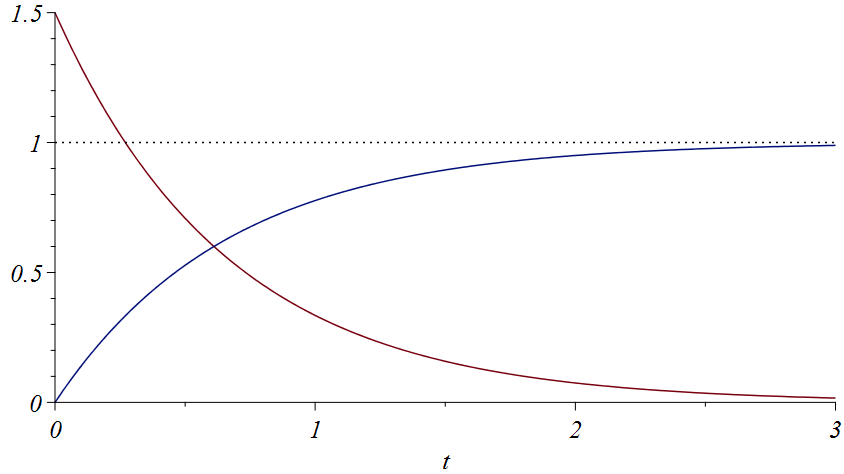
\includegraphics[width=0.7\textwidth]{images/exp-cum.png}
  \end{center}
\end{itemize}
\end{n}

\ssn{Definition}
The \emph{expected value} of a random variable $X$ with pdf $f_X(x)$ 
is given by 
\tcb 
 \[
    \EE(X) = \int_{-\infty}^\infty x \, f_X(x) \dd x.
   \]
   \etcb 
   
\noindent    
More generally, we can take the expected value of a function $g(X)$ of our random variable $X$: 
\tcb 
 \[
    \EE(g(X)) = \int_{-\infty}^\infty g(x) \, f_X(x) \dd x.
   \]
  \etcb 
 
 \noindent If the random variable $X$ takes values only in an interval $[a,b]$ then the limits of the integral can be taken to be $a$ and $b$. 
\end{n}

\ssn{Examples} 
\begin{itemize}
\item For the rod example where $f_X(x)=1/L$ on $[0,L]$, the expected value of $X$ is 
 \[
 \EE(X) =  \int_0^L  \frac1L  x \dd x = \left[ \frac{x^2}{2L}\right]_0^L = \frac{L}2, 
  \]
 which surely accords with our intuition. 
 
 Similarly (exercise)  $\EE(X^2) = L^2/3$. 
 \item 
 For the exponential distribution on $[0,\infty]$ where $f_T(t) = \lambda e^{-\lambda t}$ we have 
  \[
 \EE(T)= \int_0^\infty u \, \lambda e^{-\lambda u} \,\dd u = 
   \left[ - u e^{-\lambda u} \right]_0^\infty +
   \int_0^\infty e^{-\lambda t} \dd t = 0 + \frac1\lambda = \frac1\lambda
  \]
 where at the start we integrated by parts. 
\end{itemize}

\end{n}



\ssn{Foundations}
We will not present a completely rigorous version of the foundations of continuous probability. The fundamental difficulty is that an event will be a subset of the sample space and it needs to be a subset over which a suitable pdf can be integrated, and we do not study integration rigorously until later in the degree.  We will only consider events that are finite unions of intervals. 

Given that we assume that $f_X(x)$ is piecewise continuous,  $\int_x^x f_X(u) \dd u = 0$ and we are forced to have $\PP(X=x) = 0$ for all points $a$.   Consequently it does not matter if endpoints are included because $\PP(X<x) = \PP(X \leq x)$ and so on. 

We will assume that probabilities for events obey the fundamental properties in \S\ref{prprops} without proof.    
\end{n}

\ssn{The Gamma function} \label{guseful} 
The \emph{Gamma function} is a way of defining factorials for all positive real numbers rather than just integers. 
We define 
\tcb 
 \[
    \Gamma(z) = \int_0^\infty x^{z-1} e^{-x} \dd x, \quad \text{where $z>0$}.  
 \]
 \etcb 
\noindent 
Integrating by parts (where we differentiate the term $x^{z-1}$) we get 
 \begin{eqnarray*} 
  \Gamma(z)  &=& \int_0^\infty x^{z-1} e^{-x} \dd x \\
  &=& \left[ - x^{z-1} e^{-x}  \right]_0^\infty + 
    \int_0^\infty (z-1)x^{z-2} e^{-x} \dd x \\
    &=&  (z-1) \int_0^\infty x^{z-2} e^{-x} \dd x = 
     (z-1) \Gamma(z-1) 
 \end{eqnarray*} 
 So we see 
 \tcb
  \[
     \Gamma(z) = (z-1) \Gamma(z-1).
   \]
 \etcb 
 
 \noindent 
 Also, $\Gamma(1) = 1$ by an easy integral. So by the above, $\Gamma(2) = 1 . \Gamma(1) = 1$. And $\Gamma(3) = 2 \Gamma(2)=2$, and $\Gamma(4) = 3 \Gamma(3) = 6$. Carrying on, we see that for non-negative integers 
\tcb 
 \[
      \Gamma (n) = (n-1)! 
 \]
\etcb 
\noindent 
It is annoying that the definition of the gamma function is somehow ``off by one'' compared to the factorials, but we are stuck with it.    
\end{n}

\ssn{A useful formula} \label{guseful2} 
For $x, \lambda >0$ we have 
 \tcb 
 \[
      \int_0^\infty x^{z-1} e^{-\lambda x} \dd x = \frac{1}{\lambda^z}  \Gamma(z). 
 \]
 \etcb 
 \noindent 
This is derived by changing variables, substituting $u=\lambda x$ in the definition of the gamma function. 
\end{n} 

\ssn{Definition: The Gamma distribution}
Let $\alpha$ and $\lambda$ be positive constants. The random variable $X$ taking values in $[0,\infty)$ has a \ul{gamma distribution} and we write  $X \sim \gamm(\alpha, \lambda)$ if its pdf is  
\tcb 
 \[
    f_X(x) = \frac{\lambda^\alpha}{\Gamma(\alpha)} 
     x^{\alpha -1} e^{-\lambda x}. 
 \]
\etcb 
\noindent 
Note that when $\alpha = 1$ we have the exponential distribution that we studied earlier. 

The Gamma distribution is not a ``core'' distribution for us: we will use it for some examples, but familiarity with \emph{when} to use it is not expected. (But it is important: for example, the $\chi^2$ distribution with $v$ degrees of freedom used in statistics is $\gamm(v/2, 1/2)$.)  
\end{n} 

\ssn{Example} 
Compute $\EE(X)$ where $X \sim \gamm(z, \lambda)$.  The pdf for $X$ is thus 
 \[
   f_X(x) = \frac{\lambda^z}{\Gamma(z)} x^{z-1} e^{-\lambda x}. 
  \]
 So 
  \begin{eqnarray*} 
    \EE(X) &=& \int_0^\infty x f_X(x) \dd x \\  
    &=&  \frac{\lambda^z}{\Gamma(z)} \int_0^\infty x^z e^{-\lambda x} \dd x \\
    &=& \frac{\lambda^z}{\Gamma(z)} \frac{\Gamma(z+1)}{\lambda^{z+1}} \quad \text{(using the useful formula \S\ref{guseful2})} \\ 
  &=& \frac{z}{\lambda} \quad \text{(using final formula in \S\ref{guseful})}
  \end{eqnarray*} 

\end{n} 

\ssn{Useful and interesting integrals} 
The function $e^{-x^2}$ is fundamentally important in statistics particularly. Unfortunately there is no way of writing down its integral in terms of familiar functions.  One can however compute its integral over the whole real line by a trick. Let 
\[
    I = \int_{-\infty}^\infty e^{-x^2} \dd x.
\]
Then 
\begin{eqnarray*} 
    I^2 & = & \left(\int_{-\infty}^\infty e^{-x^2} \dd x\right) \, \left(\int_{-\infty}^\infty e^{-y^2} \dd y\right) \\
     &=& \int_{-\infty}^\infty \int_{-\infty}^\infty e^{-x^2}  e^{-y^2} \dd x \dd y  \\
     &=& \int_{r=0}^\infty \int_{\theta=0}^{2 \pi} e^{-r^2} r \dd \theta \dd r  \qquad\text{(converting to polar coordinates)}\\
     &=&   2 \pi \int_{r=0}^\infty e^{-r^2} r \dd r \\
     &=&  2 \pi \frac12 = \pi  
\end{eqnarray*} 
So 
\[
    \int_{-\infty}^\infty e^{-x^2} \dd x = \sqrt{\pi}
\]

Now consider $\Gamma(1/2)$.  It turns out we can do the integral by substituting $x = t^2$ as follows:
 \begin{eqnarray*} 
 \Gamma(1/2) & = & \int_0^\infty x^{-1/2} e^{-x} \dd x \\
  &=& \int_0^\infty t^{-1} e^{-t^2}  2 t \dd t \quad \text{(substituting)} \\
  &=&  \int_{-\infty}^\infty e^{-t^2}  \dd t \quad \text{(the integrand is even)} \\
  & = & \sqrt{\pi}.
\end{eqnarray*} 
And from $\Gamma(1/2) = \sqrt\pi$ we deduce that 
 \[
     \Gamma(3/2) = 1/2 \Gamma(1/2) = \frac{\sqrt\pi}2. 
 \]
So, if it makes sense to talk about factorials of things that are not integers, we arrive at 
 \[
      (-1/2)! \;\text{ ``$=$'' }\;  \sqrt\pi \qquad \text{and} \qquad (1/2)! \;\text{ ``$=$'' }\; \frac{\sqrt\pi}2. 
 \]
\end{n}



\subsection{Exercises and problems}

\sse 
Invent a random variable $X$ that is sufficiently simple that you can compute its expected value $\EE(X)$, the value of $\EE(x^2)$ and its cdf $F_X(x)$.   
\end{e}

\sse{}
Let $X \sim \gamm(z,\lambda)$.  Compute $\EE(X^2)$.   (Ans: $z(z+1)/\lambda^2$) 
\end{e}

\sse{}
Let $X \sim \geom(\lambda)$.  Compute $\EE(X^2)$.   (Ans: $2/\lambda^2$) 
\end{e}

\ssp{}
A room has two new light bulbs fitted and left permanently on at time $t=0$. They are the only illumination in the room. Each one independently has a failure time described by an exponential random variable $T$ with parameter $\lambda = 1$. 
\begin{enumerate}
    \item Write down the pdf, cdf and expected value of $T$.
    \item Consider a time $t=x$. What is the probability that both bulbs have failed (and so the room is dark) at the time $t=x$? 
    \item Let $X$ be the random variable which is the time that the room goes dark.  Compute the pdf of $X$ and its expected value. 
\end{enumerate}
(Hint: the second part is asking you to calculate the cdf of $X$.) 
\end{e}



\subsection{Supplementary Material about Transformations}

\ssn{Motivating problem}

You are working in a laboratory and know from experience that the result $X$ of some experiment is uniformly distributed in the range $[1,2]$. For a public presentation you want to do this experiment in a larger scale. You plan to triple the size, i.e.\ the new result $Y$ will be $Y=3 \cdot X$. To implement some safety precautions you need to know the distribution of $Y$. \\
What is the pdf of $Y$ here?

\end{n}

\ssn{Example}

Let $X \sim \unif(1,2)$ and $Y:= 3 \cdot X$. What is the pdf $f_X$?

We know from Proposition \ref{PropCdfPdf} that $f_Y(y) = \partial_y F_Y (y)$, hence we can just concentrate on finding $F_Y$.
First, we have a look at the definition $F_Y(y) = \PP (Y \leq y)$. Here we notice, that since $Y= 3X$, we can simply replace it to obtain $\PP(Y \leq y) = \PP(3X \leq y)$. Doing the equivalent transform of dividing both sides of the inequality by 3 we have $\PP(3X\leq y)= \PP(X \leq y/3)$. Notice that this is the cdf of $X$, which we know to be
$$F_X(x)= \int_{-\infty}^x \1_{\{x \in [1,2]\}} dx
= \left\{ \begin{array}{ll}
0,\quad & x < 1 \\
x-1, \quad & 1 \leq x \leq 2 \\
1, \quad & 2 < x.
\end{array}
\right.$$
Putting this together we have
\begin{align*}
F_Y(y)
&
= \PP(Y\leq y)
%\\ &
= \PP(3X \leq y)
%\\ &
= \PP \Big(X \leq \frac{y}{3} \Big)
%\\ &
= F_X \Big(\frac{y}{3} \Big)
\\ &
= \left\{ \begin{array}{ll}
0,\quad & y/3 < 1 \\
y/3-1, \quad & 1 \leq y/3 \leq 2 \\
1, \quad & 2 < y/3.
\end{array}
\right. \quad
%\\ &
= \left\{ \begin{array}{ll}
0,\quad & y < 3 \\
y/3-1, \quad & 3 \leq y \leq 6 \\
1, \quad & 6 < y.
\end{array}
\right.
\end{align*}
Differentiating, we get $f_Y(y) = \partial_y F_Y(y) = \frac13 \1_{\{ y \in [3,6] \} }$, i.e.\ $Y$ is uniformly distributed on $[3,6]$.

\


\end{n}

\ssn{Theorem}


We did the last example for a quite simple transformation and a quite simple distribution. Can we do this in general?

Let us assume that now we are given the pdf of $X$, denoted by $f_X$ and that $Y:= g(X)$ for some function $g$. We can say the following.

\tcb
Let $X$ be a continuous random variable with given pdf $f_X$ and let $g: \RR \to \RR$ be such that its inverse $g^{-1}$ exists (i.e.\ there exists a function $g^{-1}$ such that $g^{-1}(g(x)) = x$), is differentiable and monotone increasing where $f_X$ is positive. Define $Y$ as $Y:= g(X)$. Then
$$f_Y(y) 
= f_X(g^{-1}(y))  \cdot (g^{-1})'(y).
$$
\etcb

\begin{proof}
We do the exact same calculation as above. In detail it is
\begin{align*}
F_Y(y)
&
= \PP(Y\leq y)
%\\ &
= \PP(g(X) \leq y)
%\\ &
= \PP (g^{-1}(g(X)) \leq g^{-1}(y))
%\\ &
= \PP (X \leq g^{-1}(y))
%\\ &
= F_X (g^{-1}(y)),
\end{align*}
where we used that applying the inverse of $g$ on both sides gives an equivalent statement. Finally, we differentiate to obtain
\begin{align*}
f_Y(y)
&
= \partial_y F_Y(y)
\\&
= \partial_y F_X( g^{-1}(y))
\\ &
= (F_X)'(g^{-1}(y)) \cdot (g^{-1})'(y)
\\ &
= f_X(g^{-1}(y)) \cdot (g^{-1})'(y),
\end{align*}
where the chain rule was applied.
\end{proof}

Now let us have a look at two examples where $g$ does not have an increasing inverse.

\end{n}

\ssn{Example}

Let $X \sim Exp(\lambda)$, $g(x)= -a x$ for some $a > 0$ and $Y:=g(X)$.
\\
We can still use the basic calculation from above. However, the step where we formally applied the inverse of $g$ requires closer attention.
\begin{align*}
F_Y(y)
&
= \PP(Y\leq y)
%\\ &
= \PP(-aX \leq y)
\end{align*}
Here it becomes obvious that the calculation does not go the exact same way. Instead we obtain
$$ \PP(-aX \leq y) = \PP\Big(X \geq -\frac{y}{a}\Big).$$
Continuing our calculation with this slightly changed step and using that single points have probability 0, we get
\begin{align*}
F_Y(y)
&
=\PP\Big(X \geq -\frac{y}{a}\Big)
%\\&
= 1 - \PP\Big(X < -\frac{y}{a}\Big)
= 1 - \PP\Big(X < -\frac{y}{a}\Big)
= 1 - F_X\Big( -\frac{y}{a}\Big)
.
\end{align*}
Now we again can differentiate to obtain that
\begin{align*}
f_Y(y)
&= \partial_y F_Y(y)
= \partial_y \Big(1-F_X\Big(-\frac{y}{a}\Big)\Big)
= \frac1a f_X\Big(-\frac{y}{a}\Big)
= \left\{ \begin{array}{ll}
0, \quad & -\frac{y}{a} < 0 \\
\frac1a \lambda e^{-\lambda (-\frac{y}{a})}, \ & 0 \leq -\frac{y}{a}
\end{array} \right.
\\ &
= \left\{ \begin{array}{ll}
0, \quad & y > 0 \\
\frac{\lambda}{a} e^{\frac{\lambda}{a} y}, \ & 0 > y.
\end{array}
\right.
\end{align*}
Note that this is not an exponential distribution, since its mass is on the negative axes.

\end{n}

\ssn{Example}

As a final example, we have a look at what happens, if $g$ is not invertible. For this, let $g(x)= x^2$, $X \sim \unif([-1,2])$ and $Y:= g(X)$, i.e.\ $Y:= X^2$ and $F_X(x) = \frac13 (1+x) \1_{\{x \in [-1,2]\}} + \1_{\{x > 2\}}$. Starting as usual, we have
$F_Y(y)
= \PP ( X^2 \leq y ).$ Here we see the problem, that we cannot invert, since left from $0$ the inverse is $-\sqrt{\cdot}$, while on the right it is $\sqrt{\cdot}$. Instead, we find the equivalent formulation $\vert X \vert \leq \sqrt{y}$. However, we need to require for this that $y \geq 0$. Because $X^2 \geq 0$, this is no problem and just means that $F_Y(y) =0$ for all $y<0$. Collecting all of that, we progress to
$$ F_Y(y) 
= \PP ( X^2 \leq y ) 
= \PP ( \vert X \vert \leq \sqrt{y}) \1_{\{y \geq 0\}}
= \PP ( -\sqrt{y} \leq X \leq \sqrt{y}) \1_{\{y \geq 0\}}
.
$$
Replacing the probability with the cdf this reads as
$$ F_Y(y)
= \PP ( -\sqrt{y} \leq X \leq \sqrt{y}) \1_{\{y \geq 0\}}
= (F_X(\sqrt{y})-F_X(-\sqrt{y}))\1_{\{y \geq 0\}}
.
$$
Now we can use the explicit expression for $F_X$ from above to get
\begin{align*}
F_Y(y)
&
=
\left[ \frac13 (1+\sqrt{y}) \1_{\{\sqrt{y} \in [-1,2]\}} + \1_{\{\sqrt{y} > 2\}} - \frac13 (1-\sqrt{y}) \1_{\{-\sqrt{y} \in [-1,2]\}} - \1_{\{-\sqrt{y} > 2\}} \right] \1_{\{y \geq 0\}}
,
\end{align*}
which looks quite intimidating. However, in a first step we can simplify it, by removing all cases where $\sqrt{y}$ would have to be negative and as a second step, we split it up into the disjoint cases $\sqrt{y} \in [0,1]$, $\sqrt{y} \in [1,2]$ and $\sqrt{y} > 2$. Thus, we have
\begin{align*}
F_Y(y)
&
=
\left[ \frac13 (1+\sqrt{y}) \1_{\{\sqrt{y} \in [0,2]\}} + \1_{\{\sqrt{y} > 2\}} + \frac13 (\sqrt{y}-1) \1_{\{\sqrt{y} \in [0,1]\}} - 0 \right] \1_{\{y \geq 0\}}
\\ &
=
\left\{ \begin{array}{ll}
0, \quad & y < 0 \\
\frac13 (1+\sqrt{y}) + \frac13 (\sqrt{y}-1), \quad & 0 \leq \sqrt{y} \leq 1\\
\frac13 (1+\sqrt{y}), \quad & 1 < \sqrt{y} \leq 2 \\
1, \quad & 2 < \sqrt{y}
\end{array}
\right.
\\ &
=
\left\{ \begin{array}{ll}
0, \quad & y < 0 \\
\frac23 \sqrt{y}, \quad & 0 \leq y \leq 1\\
\frac13 (1+\sqrt{y}), \quad & 1 < y \leq 4 \\
1, \quad & 4 < y
\end{array}
\right.
.
\end{align*}
A quick sanity check is, whether this is actually a non-decreasing function as it should be. Since every single part is non-decreasing, we only need to have a look at the border cases $y=0,1,4$ which all turn out to be fine.

So finally, we only have to differentiate to obtain $f_Y$. Doing so we get
\begin{align*}
f_Y(y)
= \partial_y F_Y(y)
= \left\{ \begin{array}{ll}
0, \quad & y < 0 \\
\frac{1}{3 \sqrt{y}}, \quad & 0 \leq y \leq 1\\
\frac{1}{6 \sqrt{y}}, \quad & 1 < y \leq 4 \\
0, \quad & 4 < y
\end{array}
\right.
.
\end{align*}

\end{n}


\subsection{Exercises and problems}

\sse 
The random variable $X \sim \gamma(2,\lambda)$ and $Y:= \ln (X)$. Find the pdf $f_Y$. \\ (Ans.: $f_Y(y) = \frac{\lambda^2}{2} e^y e^{-\lambda e^y} \1_{\{y > 0\}}$ )
\end{e}

\sse{}
Show that for any continuous random variable $X$ it is true that $F_X(X) \sim \unif(0,1)$. 
\end{e}

\ssp{}
Let $X$ have any continuous distribution and let $Y \sim \unif(0,1)$. Show that $Z:= F_X^{-1} (Y)$ has the same distribution as $X$, i.e.\ that $F_Z = F_X$.
\end{e}

\sse{}
Let $X \sim \expo(\lambda)$.  Compute $F_Y$ for $Y:= X^2$.   (Ans: $(1-e^{-\lambda \sqrt{y}}) \1_{\{ y \geq 0 \}}$) 
\end{e}

